\addsection{Expansion Content}{\images/pathfinding.png}

\begin{figure}[h]
  \begin{minipage}[t]{0.48\textwidth}
    \vspace{0pt}
    \subsection*{Schools of magic}
    Most expansions have cards which refer to schools of magic.
    All spell cards belong to one school: either air, fire, earth or water.
    There are multiple different cards and effects that interact with the schools in some way.
    The “magic arrow” spell can be considered to belong to every school but can only benefit from bonuses for a single school at a time.
    If relevant, you must select which school the magic arrow belongs to when casting it.
    Hero specialty cards are not spells even though some of them have a school of magic.
  \end{minipage}
  \begin{minipage}[t]{0.48\textwidth}
    \vspace{0pt}
    \centering
    \minipage[b]{0.5\textwidth}
      \centering
      
\includegraphics[scale=0.17]{\images/school_of_fire.png}
      \caption{{\textit{\textbf{\textcolor{darkcandyapplered}{School of Fire}}}}}
    \endminipage
    \minipage[b]{0.5\textwidth}
      \centering
      
\includegraphics[scale=0.17]{\images/school_of_water.png}
      \caption{{\textit{\textbf{\textcolor{darkcandyapplered}{School of Water}}}}}
    \endminipage
    \hfill\allowbreak%
    \bigbreak
    \minipage[b]{0.5\textwidth}
      \centering
      
\includegraphics[scale=0.17]{\images/school_of_air.png}
      \caption{{\textit{\textbf{\textcolor{darkcandyapplered}{School of Air}}}}}
    \endminipage
    \minipage[b]{0.5\textwidth}
      \centering
      
\includegraphics[scale=0.17]{\images/school_of_earth.png}
      \caption{{\textit{\textbf{\textcolor{darkcandyapplered}{School of Earth}}}}}
    \endminipage
  \end{minipage}
\end{figure}

\subsection*{Permanent cards}
Added by the stretch goals and Rampart expansions, explained \hyperlink{Playerdecks}{here}.

\begin{figure}[h]
  \begin{minipage}[t]{0.5\textwidth}
    \vspace{0pt}
    \subsection*{War machines}
    Added by the Rampart expansion.
    War machines are permanent cards that can be bought at either a trading post or a war machine factory.
    If you buy one at the trading post, you cannot use any of the other normal functions of that field during that visit.
    War machines are also more expensive at the trading post.
    \textit{I don't currently know if these have a player card back and are added to your hand like normal?}\par
    \smallskip
    \raggedright\textbf{War Machine Factory}
    \shadowimage[width=0.8\textwidth]{\images/war_machine_factory.jpg}
      \caption{\scriptsize Category: \scriptsize\textbf{Revisitable}\\This location allows a Hero to buy a War Machine.}
  \end{minipage}
  \begin{minipage}[t]{0.4\textwidth}
    \vspace{0pt}
    \centering
    \begin{scriptsize}
      \begin{tikzpicture}
        \draw (0, 0) node[inner sep=0] {\makebox[\textwidth][c]{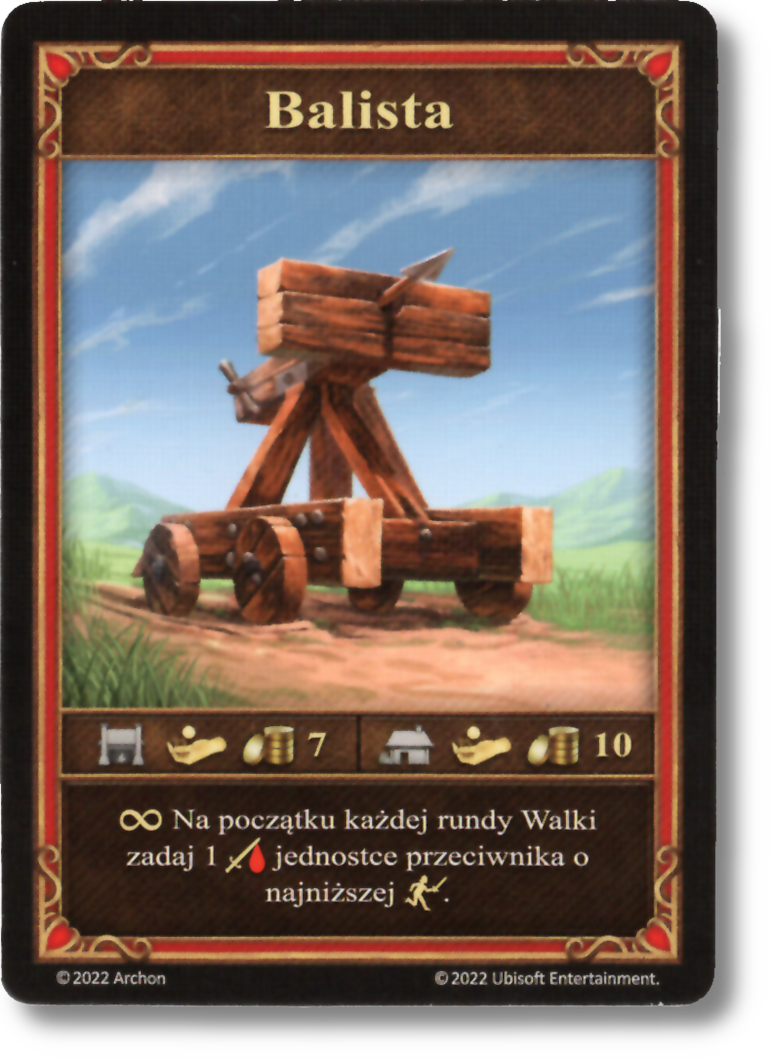
\includegraphics[width=0.8\textwidth]{\images/war_machine.png}}};
        \draw (0.8, 3) node {\encircle{\phantom{.}1\phantom{.}}};
        \draw (0, -2.8) node {\encircle{\phantom{.}2\phantom{.}}};
        \draw (-1.2, -1.7) node {\encircle{\phantom{.}3\phantom{.}}};
        \draw (0.9, -1.7) node {\encircle{\phantom{.}4\phantom{.}}};
      \end{tikzpicture}
    \end{scriptsize}
    \break
    \footnotesize{\textbf{\textit{\textcolor{darkcandyapplered}{War Machine Card}}}}
    \scriptsize
    \begin{multicols}{2}
      \begin{itemize}
        \item[\textbf{1.}] \textbf{Name}
        \item[\textbf{2.}] \textbf{Effect}
        \item[\textbf{\phantom{.}}] \phantom{.}
        \item[\textbf{3.}] \textbf{War Machine Factory cost}
        \item[\textbf{4.}] \textbf{Trading Post cost}
      \end{itemize}
    \end{multicols}
  \end{minipage}
\end{figure}

\begin{wrapfigure}{r}{0.5\textwidth}
  \vspace{0pt}
  \centering
  \begin{scriptsize}
    \begin{tikzpicture}
      \draw (0, 0) node[inner sep=0] {\makebox[0.5\textwidth][c]{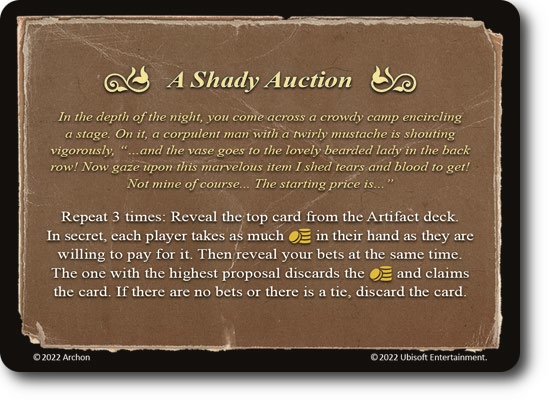
\includegraphics[width=0.4\textwidth]{\images/event_card.png}}};
      \draw (1, 1.6) node {\encircle{\phantom{.}1\phantom{.}}};
      \draw (-2, 0.4) node {\encircle{\phantom{.}2\phantom{.}}};
      \draw (2.5, -1.1) node {\encircle{\phantom{.}3\phantom{.}}};
    \end{tikzpicture}
  \end{scriptsize}
  \break
  \footnotesize{\textbf{\textit{\textcolor{darkcandyapplered}{Event Card}}}}
  \scriptsize
  \begin{multicols}{2}
    \begin{itemize}
      \item[\textbf{1.}] \textbf{Name}
      \item[\textbf{2.}] \textbf{Fluff}
      \item[\textbf{3.}] \textbf{Effect}
      \item[\textbf{\phantom{.}}] \phantom{.}
    \end{itemize}
  \end{multicols}
\end{wrapfigure}
\subsection*{Events}
Added by the Fortress expansion.
Event cards may be used in games with more than one player.
Shuffle the event deck during set up.
At the start of each resource round (except the first round), draw and read the next event card after receiving resources.
The first event is drawn by the starting player.
Change this player in a clockwise order every time a new event is drawn.
Resolve any effects in clockwise order starting with the player who drew the card.
Any cards which were revealed as a part of resolving an event should be shuffled back into their respective decks afterwards.

\begin{wrapfigure}{r}{0.5\textwidth}
  \begin{center}
  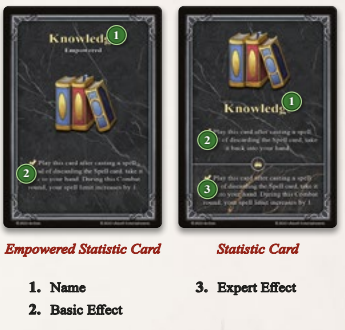
\includegraphics[width=0.48\textwidth]{\images/empowered_statistics.png}
  \end{center}
\end{wrapfigure}
\subsection*{Empowered statistic cards}
Added by the Inferno expansion.
These cards are more powerful versions of the normal statistics cards.
They have only one effect which is identical to the normal statistic's expert effect, but does not require using your \includesvg[height=10px]{\svgs/expert.svg}.

\subsection*{Summoning}
Some cards from the Inferno expansion may summon units during combat.
Place the summoned unit adjacent to the summoning unit.
Summoned units activate in the round they were summoned if their initiative is lower or equal to the initiative of the currently activated unit.
Otherwise, treat them as if they already activated this combat round.
After combat, unless stated otherwise, the summoned units are added to your unit deck.

\begin{wrapfigure}{r}{0.5\textwidth}
  \begin{center}
    \textbf{Random Town}
    \shadowimage[width=0.48\textwidth]{\images/random_town.jpg}
    \caption{\scriptsize Category: \scriptsize\textbf{Flaggable}}
  \end{center}
\end{wrapfigure}
\subsection*{Random town}
Added by the Inferno expansion.
When this field is revealed, all players roll 2 \includesvg[height=10px]{\svgs/resource_die.svg}.
The highest roller chooses an unused faction.
The random town is defended by units from that faction.
They have a pack of bronze, two packs of silver, and two "fews" of gold units.
Flagging it increases gold production by 10, which is also gained immediately if you are the first to flag it.
